\section{Summary Statistics}
\label{sec:appendixsumstat}

Table~\ref{tab:summarytab1} and Table~\ref{tab:summarytab2} display univariate summary statistics from the primary dataset. We display the mean, interquartile range, and the range (as defined by the maximum value minus the minimum value) for the unadjusted dataset, the heterogeneous adjustment, and the homogeneous adjustment. We see that in general the covariate adjustments reduce the variability in the data. However, we also see that the range sometimes increases drastically, particularly for the untreated dataset. Table~\ref{tab:extreme1} displays the overall number of CPUMAs whose adjusted values fall outside of the range of the unadjusted data. We emphasize that we only use the untreated data for the heterogeneous treatment effect analysis in Appendix~\ref{ssec:varselection}. We also calculate these adjustments when leaving out each state one at a time from the primary dataset to calculate our secondary variance estimates; these results are available on request. 

\begin{table}[h!]
\centering
\caption{Univariate summary statistics on adjusted data by treatment group (1) \\ (Mean, IQR, Range)}\label{tab:summarytab1}
\begin{tabular}{rllll}
  \hline
Treatment & Variable & No adjustment & Heterogeneous & Homogeneous \\ 
  \hline
0 & Age: 19-29 Pct & (24.8, 5.5, 48.7) & (24.8, 5.4, 47.5) & (24.8, 5.4, 47.8) \\ 
  1 & Age: 19-29 Pct & (24.5, 6, 30.9) & (24.5, 5.9, 29) & (24.5, 5.9, 29) \\ 
  0 & Age: 30-39 Pct & (20.6, 2.6, 18.4) & (20.6, 2.5, 17.3) & (20.6, 2.5, 17.2) \\ 
  1 & Age: 30-39 Pct & (20.9, 3.4, 20.9) & (20.9, 3.1, 19.1) & (20.9, 3.1, 19.4) \\ 
  0 & Age: 40-49 Pct & (22, 2.5, 19.5) & (21.9, 2.4, 51.6) & (22, 2.3, 18.5) \\ 
  1 & Age: 40-49 Pct & (22.2, 2.5, 15.4) & (22.2, 2.3, 13.7) & (22.2, 2.2, 13.7) \\ 
  0 & Avg Adult to Household Ratio & (139.7, 18.7, 156.8) & (139.7, 18.9, 153.7) & (139.7, 18.9, 154.1) \\ 
  1 & Avg Adult to Household Ratio & (151, 27.2, 174.3) & (151, 27.2, 173.8) & (151, 27.2, 173.3) \\ 
  0 & Avg Pop Growth & (100.3, 1.7, 14.3) & (99.9, 1.1, 430.7) & (100.3, 1, 5.1) \\ 
  1 & Avg Pop Growth & (100.3, 1.9, 13.7) & (100.3, 1.2, 6.2) & (100.3, 1.2, 6.5) \\ 
  0 & Children: Missing Pct & (13.7, 7.4, 36.2) & (13.8, 7.3, 38) & (13.7, 7.3, 35.6) \\ 
  1 & Children: Missing Pct & (10.5, 6.6, 41) & (10.5, 6.5, 40.8) & (10.5, 6.5, 40.5) \\ 
  0 & Children: One Pct & (10.4, 2.5, 13) & (10.1, 2.2, 249.2) & (10.4, 2.1, 12.2) \\ 
  1 & Children: One Pct & (11.1, 3.1, 14.3) & (11.1, 2.8, 12.3) & (11.1, 2.8, 12.5) \\ 
  0 & Children: Three or More Pct & (5.2, 2.2, 25.3) & (5.2, 2.1, 59.2) & (5.2, 2.2, 23.2) \\ 
  1 & Children: Three or More Pct & (5.2, 2, 14.1) & (5.2, 1.7, 13.5) & (5.2, 1.7, 13.3) \\ 
  0 & Children: Two Pct & (8.9, 2.8, 15) & (9.1, 2.5, 190.4) & (8.9, 2.5, 15) \\ 
  1 & Children: Two Pct & (9.7, 3.5, 15) & (9.7, 3.3, 13.5) & (9.7, 3.2, 13.6) \\ 
  0 & Citizenship Pct & (93.6, 5.9, 39.8) & (93.6, 5.8, 39.7) & (93.6, 5.9, 39.3) \\ 
  1 & Citizenship Pct & (90, 11.9, 57.1) & (90, 11.8, 55.4) & (90, 11.7, 55.7) \\ 
  0 & Disability Pct & (11.9, 5, 22.1) & (11.9, 4.8, 22.5) & (11.9, 4.8, 20.7) \\ 
  1 & Disability Pct & (10.5, 5.3, 28.6) & (10.4, 5.3, 26.7) & (10.5, 5.4, 27.2) \\ 
  0 & Educ: HS Degree Pct & (29.6, 8.8, 42.7) & (29.6, 8.8, 40.6) & (29.6, 8.8, 41.1) \\ 
  1 & Educ: HS Degree Pct & (26.3, 10.7, 43.2) & (26.3, 10.6, 41.8) & (26.3, 10.6, 42) \\ 
  0 & Educ: Less than HS Pct & (11.8, 7.1, 30) & (11.8, 6.9, 30.2) & (11.8, 7, 30.3) \\ 
  1 & Educ: Less than HS Pct & (11.4, 7.7, 45.3) & (11.4, 7.5, 45) & (11.4, 7.4, 44.6) \\ 
  0 & Educ: Some College Pct & (33.8, 5.6, 42.9) & (33.8, 5.1, 64.3) & (33.8, 5.1, 42.2) \\ 
  1 & Educ: Some College Pct & (33.5, 7.9, 34.2) & (33.5, 7.5, 32.9) & (33.5, 7.4, 33) \\ 
  0 & Female Pct & (50.5, 1.6, 15.8) & (50.5, 1.5, 14.9) & (50.5, 1.5, 15.1) \\ 
  1 & Female Pct & (50.1, 1.6, 15.4) & (50.1, 1.4, 14.2) & (50.1, 1.5, 14.2) \\ 
  0 & Foreign Born Pct & (10.5, 8.8, 63.2) & (10.5, 8.9, 62.9) & (10.5, 8.9, 62.7) \\ 
  1 & Foreign Born Pct & (18.1, 22.4, 76) & (18.1, 22.2, 75.2) & (18.1, 22.2, 75.4) \\ 
  0 & Hispanic Pct & (11.4, 10.2, 93.9) & (11.5, 10.2, 93.8) & (11.4, 10.2, 93.8) \\ 
  1 & Hispanic Pct & (15.9, 17.7, 97.2) & (15.9, 17.7, 97) & (15.9, 17.7, 97) \\ 
  0 & Inc Pov: $<$ 138 Pct & (22, 8.8, 42.8) & (22, 8.8, 41) & (22, 8.7, 41.8) \\ 
  1 & Inc Pov: $<$ 138 Pct & (20, 11.9, 45.6) & (20, 11.8, 44.8) & (20, 11.8, 43.9) \\ 
  0 & Inc Pov: 139-299 Pct & (27.4, 5.1, 27.9) & (27, 5, 328.3) & (27.4, 4.8, 26.7) \\ 
  1 & Inc Pov: 139-299 Pct & (24.9, 8.4, 34.2) & (24.9, 7.9, 34.2) & (24.9, 7.8, 34.1) \\ 
  0 & Inc Pov: 300-499 Pct & (24.2, 4.8, 21) & (24.7, 4.8, 500.5) & (24.2, 4.5, 18.4) \\ 
  1 & Inc Pov: 300-499 Pct & (23.6, 5.5, 23) & (23.6, 4.9, 22.2) & (23.6, 4.9, 22.2) \\ 
  0 & Inc Pov: 500 + Pct & (23.7, 9.9, 51.9) & (23.5, 9.7, 180.7) & (23.7, 9.7, 52.5) \\ 
  1 & Inc Pov: 500 + Pct & (29.3, 18.5, 69.1) & (29.3, 18.5, 68.1) & (29.3, 18.5, 68) \\ 
  0 & Married Pct & (51.5, 9.1, 59.7) & (51.6, 8.9, 116.7) & (51.5, 9.1, 59.5) \\ 
  1 & Married Pct & (50.7, 9.4, 45.1) & (50.7, 9, 44.1) & (50.7, 9.1, 44.2) \\ 
  0 & Race: White Pct & (77.8, 22.2, 90.5) & (77.8, 22.1, 90.2) & (77.8, 22.1, 90.4) \\ 
  1 & Race: White Pct & (73.8, 25.4, 91.9) & (73.8, 25.5, 91.7) & (73.8, 25.5, 91.8) \\ 
  0 & Republican Governor 2013 & (95.9, 0, 100) & (95.9, 0, 100) & (95.9, 0, 100) \\ 
  1 & Republican Governor 2013 & (31.1, 100, 100) & (31.1, 100, 100) & (31.1, 100, 100) \\ 
  0 & Republican Lower Leg Control 2013 & (98.8, 0, 100) & (98.8, 0, 100) & (98.8, 0, 100) \\ 
  1 & Republican Lower Leg Control 2013 & (24.1, 0, 100) & (24.1, 0, 100) & (24.1, 0, 100) \\ 
  0 & Republican Total Control 2013 & (91.1, 0, 100) & (91.1, 0, 100) & (91.1, 0, 100) \\ 
  1 & Republican Total Control 2013 & (19.8, 0, 100) & (19.8, 0, 100) & (19.8, 0, 100) \\ 
   \hline
\end{tabular}
\end{table}

\begin{table}[h!]
\centering
    \caption{Univariate summary statistics on adjusted data by treatment group (2)\\ (Mean, IQR, Range)}
    \label{tab:summarytab2}
\begin{tabular}{rllll}
  \hline
Treatment & Variable & No adjustment & Heterogeneous & Homogeneous \\ 
  \hline
  0 & Student Pct & (11.5, 3.9, 41) & (11.4, 3.9, 71.4) & (11.5, 3.8, 41.3) \\ 
  1 & Student Pct & (11.7, 3.4, 29.5) & (11.7, 3.5, 28.1) & (11.7, 3.5, 28) \\ 
  0 & Unemployed Pct 2011 & (9.4, 4.6, 21.7) & (9.4, 4, 32.7) & (9.4, 4, 19.1) \\ 
  1 & Unemployed Pct 2011 & (10.2, 4.6, 25.5) & (10.2, 3.9, 23.8) & (10.2, 3.9, 22.5) \\ 
  0 & Unemployed Pct 2012 & (8.8, 4.2, 22.4) & (8.5, 3.6, 289) & (8.8, 3.6, 18.6) \\ 
  1 & Unemployed Pct 2012 & (9.4, 4.5, 28.3) & (9.4, 4.3, 23.6) & (9.4, 4.3, 23.5) \\ 
  0 & Unemployed Pct 2013 & (8, 3.7, 19) & (8.2, 3.4, 233.9) & (8, 3.4, 17.6) \\ 
  1 & Unemployed Pct 2013 & (8.4, 3.6, 23.4) & (8.4, 3.5, 20.1) & (8.4, 3.5, 20.5) \\ 
  0 & Uninsured Pct 2011 & (22.7, 10.5, 51.4) & (21.7, 10.1, 1212.7) & (22.7, 9.3, 49.6) \\ 
  1 & Uninsured Pct 2011 & (19.6, 11.2, 59) & (19.7, 10.9, 51.8) & (19.6, 10.9, 52.5) \\ 
  0 & Uninsured Pct 2012 & (22.4, 9.3, 49.5) & (23.2, 9.4, 749.3) & (22.4, 9.2, 47.8) \\ 
  1 & Uninsured Pct 2012 & (19.4, 9.9, 50.6) & (19.4, 10.1, 49.7) & (19.4, 10.3, 50.2) \\ 
  0 & Uninsured Pct 2013 & (22, 10.1, 50.1) & (22.6, 9.4, 520.7) & (22, 9.3, 49.3) \\ 
  1 & Uninsured Pct 2013 & (19, 11.2, 49.9) & (19, 10.3, 48.2) & (19, 10.5, 48.7) \\ 
  0 & Urban Pct & (74.6, 39.2, 85.7) & (74.6, 39.2, 85.7) & (74.6, 39.2, 85.7) \\ 
  1 & Urban Pct & (82.9, 31.3, 91.3) & (82.9, 31.3, 91.3) & (82.9, 31.3, 91.3) \\ 
  \hline
\end{tabular}
\end{table}

Table~\ref{tab:extreme1} displays the frequency that the adjusted covariates fell outside of the support of the unadjusted dataset for the (control, treatment) groups. We see that that frequency is higher for our heterogeneous adjustment than the homogeneous adjustment, though the counts are low in either case. The counts are also slightly higher in the control group than the treated group; this may be a function of the smaller number of CPUMAs for the control versus the treated group $(n_0 = 411; n_1 = 515)$. We also note that these tables include 4 CPUMAs from New Hampshire that we include when conducting the covariate adjustment procedure; however, we exclude New Hampshire from the pool of treated states when computing our weights.

\begin{table}[h!]
\centering
    \caption{Frequency of ``extreme'' covariate adjustments by treatment group \\ (number in control group, number in treated group)}
    \label{tab:extreme1}
\begin{tabular}{lll}
  \hline
Variables & Heterogeneous & Homogeneous \\ 
  \hline
Age: 19-29 Pct & (0, 0) & (0, 0) \\ 
  Age: 30-39 Pct & (0, 0) & (0, 0) \\ 
  Age: 40-49 Pct & (2, 0) & (0, 0) \\ 
  Avg Adult to Household Ratio & (0, 0) & (0, 0) \\ 
  Citizenship Pct & (2, 1) & (1, 0) \\ 
  Disability Pct & (1, 2) & (0, 2) \\ 
  Educ: HS Degree Pct & (0, 0) & (0, 0) \\ 
  Educ: Less than HS Pct & (1, 1) & (2, 1) \\ 
  Educ: Some College Pct & (1, 0) & (0, 0) \\ 
  Female Pct & (0, 0) & (0, 0) \\ 
  Foreign Born Pct & (0, 1) & (0, 1) \\ 
  Uninsured Pct 2011 & (4, 0) & (0, 0) \\ 
  Uninsured Pct 2012 & (3, 1) & (0, 1) \\ 
  Uninsured Pct 2013 & (4, 0) & (1, 1) \\ 
  Hispanic Pct & (1, 0) & (1, 0) \\ 
  Inc Pov: $<$ 138 Pct & (2, 1) & (2, 1) \\ 
  Inc Pov: 139-299 Pct & (4, 1) & (1, 1) \\ 
  Inc Pov: 300-499 Pct & (3, 0) & (0, 0) \\ 
  Inc Pov: 500 + Pct & (4, 0) & (2, 0) \\ 
  Married Pct & (3, 0) & (1, 0) \\ 
  Children: Missing Pct & (2, 1) & (1, 1) \\ 
  Children: One Pct & (4, 0) & (0, 0) \\ 
  Avg Pop Growth & (3, 0) & (0, 0) \\ 
  Race: White Pct & (1, 1) & (1, 1) \\ 
  Student Pct & (2, 0) & (1, 0) \\ 
  Children: Three or More Pct & (3, 2) & (2, 1) \\ 
  Children: Two Pct & (4, 1) & (1, 1) \\ 
  Unemployed Pct 2011 & (2, 0) & (0, 0) \\ 
  Unemployed Pct 2012 & (2, 0) & (0, 0) \\ 
  Unemployed Pct 2013 & (3, 0) & (0, 0) \\ 
   \hline
\end{tabular}
\end{table}

Figure~\ref{fig:corrmatrix} displays the Pearson's correlation coefficients for the bivariate relationships between the covariates on the unadjusted dataset. The relationships appear quite similar when using the adjusted datasets and are available upon request.

\begin{figure}[h!]
\begin{center}
    \caption{Correlation matrix (unadjusted covariates)}
    \label{fig:corrmatrix}
    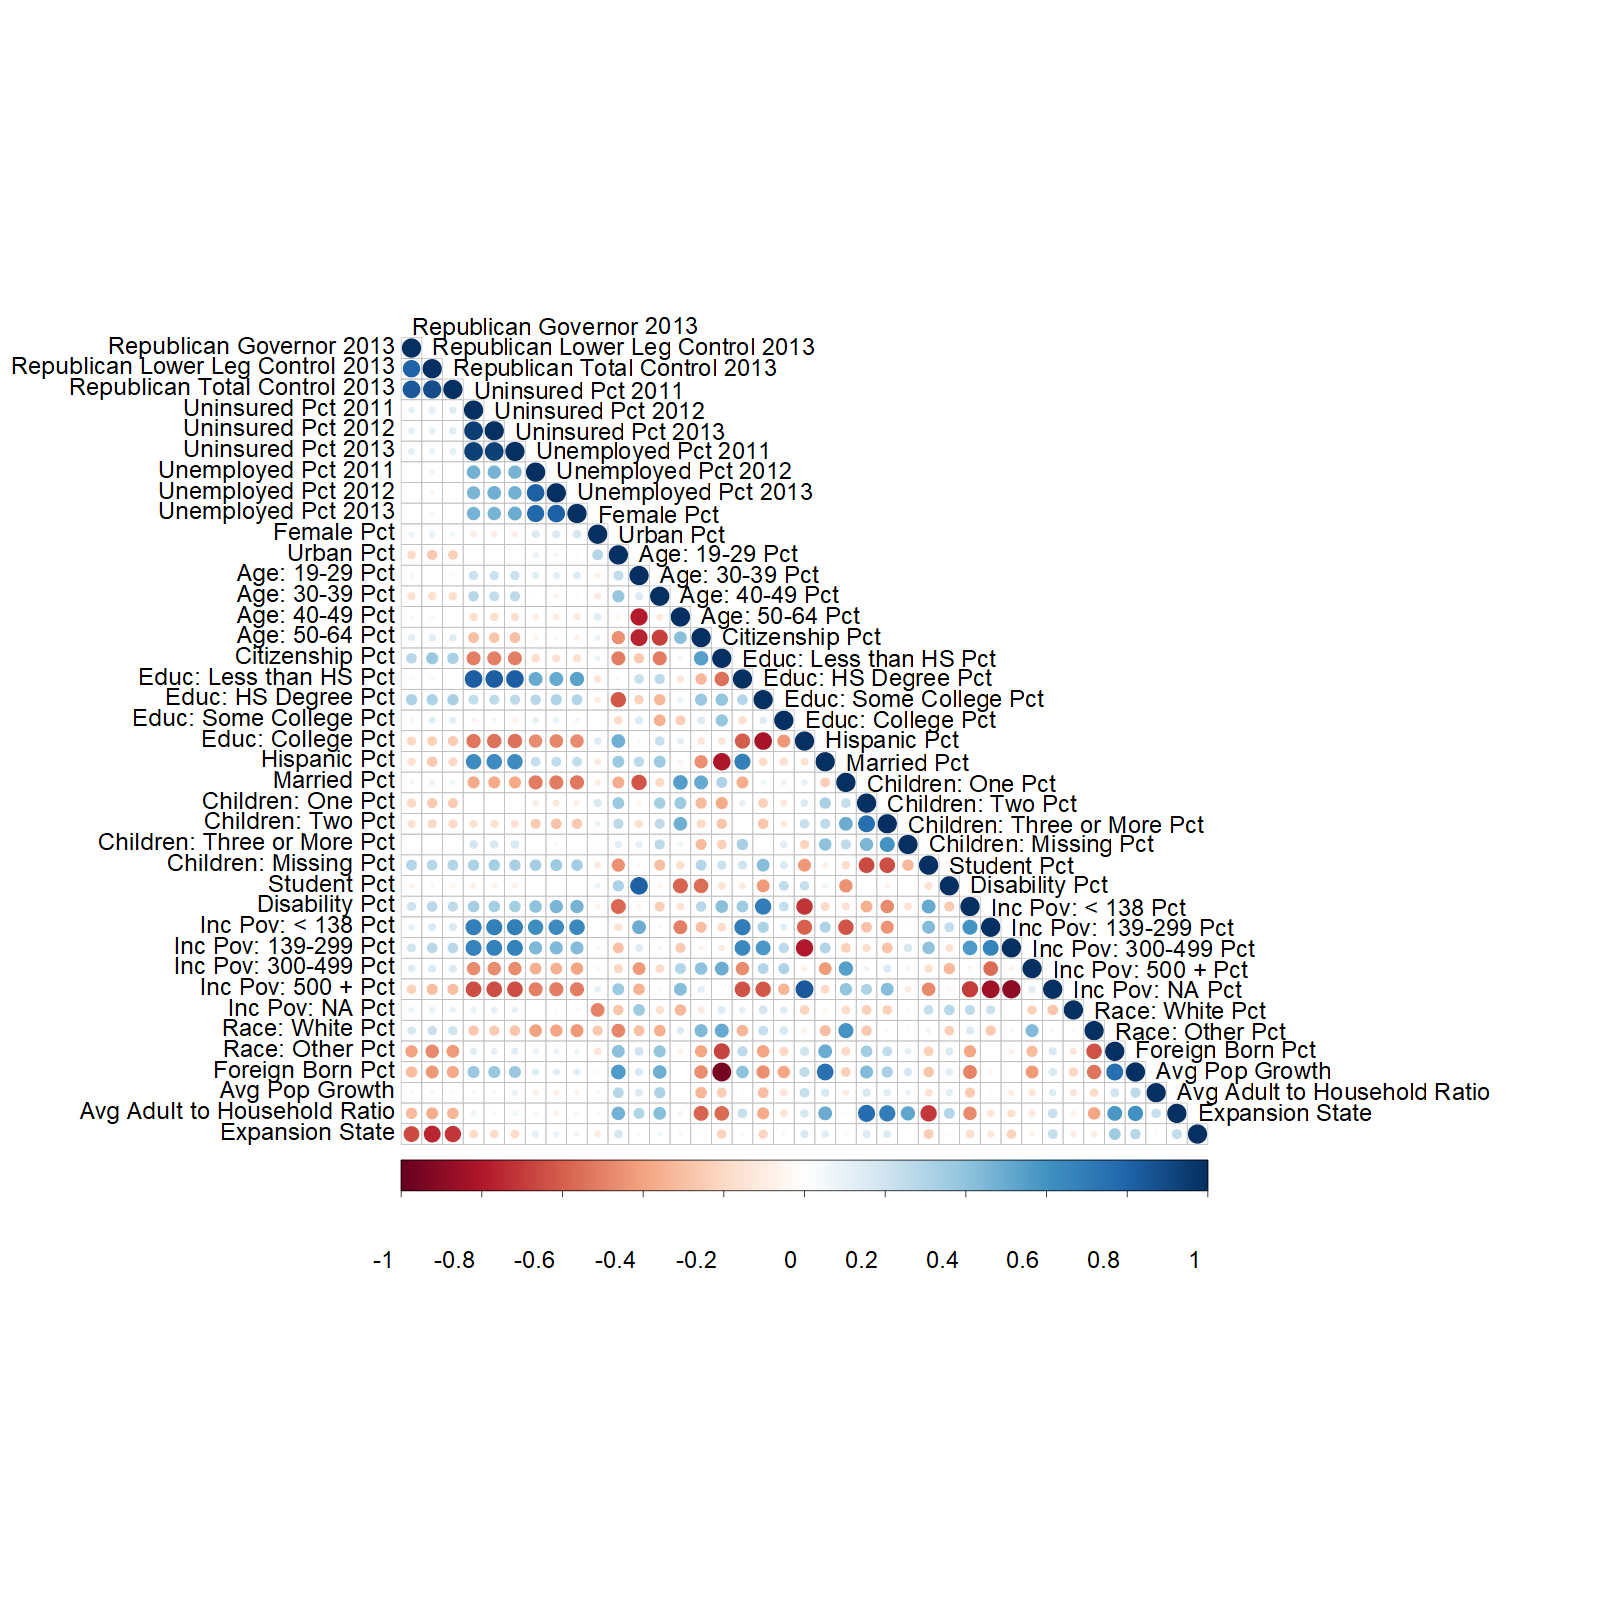
\includegraphics[scale=0.6]{01_Plots/correlation-plot-c1-sigma-zero.png}
\end{center}
\end{figure}

\clearpage